%%%%%%%%%%%%%%%%%%%%%%%%%%%%%%%%%%%%%%%%%%%%%%%%%%%%%%%%%%%%%%%%%%%%%%%%%%%%%%%%
%%%%%%%%%%%%%%%%%%%%%%%%%%%%% IMPORTS AND SETTINGS %%%%%%%%%%%%%%%%%%%%%%%%%%%%%
%%%%%%%%%%%%%%%%%%%%%%%%%%%%%%%%%%%%%%%%%%%%%%%%%%%%%%%%%%%%%%%%%%%%%%%%%%%%%%%%

% General settings
\documentclass[11pt,a4paper,notitlepage]{article}

% Misc includes
\usepackage{array}
\usepackage{xcolor}
\usepackage{longtable}

% For title + abstract page
\usepackage{titling}

% For table of contents with links
\usepackage{hyperref}
\hypersetup
{
    colorlinks,
    citecolor=black,
    filecolor=black,
    linkcolor=black,
    urlcolor=blue
}
\usepackage{ulem}

% For images
\usepackage{graphicx}
\usepackage{subfig}

% For quotes
\usepackage[english]{babel}
\usepackage[autostyle, english = american]{csquotes}
\MakeOuterQuote{"}

% For including code
\usepackage{listings}
\usepackage{color}
\definecolor{dkgreen}{rgb}{0,0.6,0}
\definecolor{gray}{rgb}{0.5,0.5,0.5}
\definecolor{mauve}{rgb}{0.58,0,0.82}
\lstset{
  language=Java,
  aboveskip=3mm,
  belowskip=3mm,
  showstringspaces=false,
  columns=flexible,
  basicstyle={\small\ttfamily},
  numbers=none,
  numberstyle=\tiny\color{gray},
  keywordstyle=\color{blue},
  commentstyle=\color{dkgreen},
  stringstyle=\color{mauve},
  breaklines=true,
  breakatwhitespace=true,
  tabsize=3,
  %frame=single,
  rulesepcolor=\color{gray},
  rulecolor=\color{black}
}

% Math
\usepackage{amssymb,amsmath}
\setlength{\thinmuskip}{3\thinmuskip}
\setlength{\medmuskip}{3\medmuskip}
\setlength{\thickmuskip}{3\thickmuskip}

% Document title data
\title{\Large{TODO\\2015-2016}\\\Huge{TODO}}
\author{836897 Simone Graziussi}
\date{TODO}



%%%%%%%%%%%%%%%%%%%%%%%%%%%%%%%%%%%%%%%%%%%%%%%%%%%%%%%%%%%%%%%%%%%%%%%%%%%%%%%%
%%%%%%%%%%%%%%%%%%%%%%%%%%%%%%%% DOCUMENT START %%%%%%%%%%%%%%%%%%%%%%%%%%%%%%%%
%%%%%%%%%%%%%%%%%%%%%%%%%%%%%%%%%%%%%%%%%%%%%%%%%%%%%%%%%%%%%%%%%%%%%%%%%%%%%%%%

\begin{document}

\sloppy

%............................................................................%
%................................ TITLE PAGE ................................%
%............................................................................%

\begin{titlingpage}
    \maketitle
    \begin{abstract}
        \large{TODO}
    \end{abstract}
\end{titlingpage}


%..............................................................................%
%............................. TABLE OF CONTENTS ..............................%
%..............................................................................%

\newpage
\tableofcontents
\newpage


%..............................................................................%
%................................... INTRO ....................................%
%..............................................................................%

\part{Introduction}

\section{Abstract}

\section{Testing}

\section{Android}

\section{Android Testing State of the Art}

\section{Introduction to Events}

\section{Background/Motivation}



%..............................................................................%
%.................................. LIFECYCLE .................................%
%..............................................................................%

\part{Lifecycle Testing}


\section{Lifecycle}

\subsection{Component Lifecycle}

\subsection{Lifecycle Problems}

\subsection{Existing Lifecycle Testing}



\section{Static Analysis}

\subsection{Static Program Analysis}

\subsection{Android Lint}

\subsection{Custom Android Lint Checks}

\subsection{Static Lifecycle Checks}

\subsubsection{Target Components}

\subsubsection{Design}

\subsubsection{Implementation}

\subsubsection{Evaluation}



\section{Dynamic Analysis}

\subsection{Design}

\subsection{Implementation}

\subsection{Evaluation}

aaa

%..............................................................................%
%.................................... EVENTS ..................................%
%..............................................................................%

\part{Event-based Testing}



\section{Event-based Systems}

\subsection{Events in Android}

\subsection{Problems with Events}

\subsection{Existing Event Testing}



\section{Temporal Assertions Language}

\subsection{Consistency Checks}

\subsection{Checks on Single Events}

\subsubsection{Can Happen Only After}

\begin{center}
\bgroup
\def\arraystretch{1.5}%
\begin{longtable}{ | m{0.3cm} | m{15cm} | }
  \hline
  
  \rotatebox[origin=c]{90}{\textbf{ Structure }} & 
  
  	\begin{lstlisting}
	anEventThat(m1).canHappenOnlyAfter(anEventThat(m2))
	\end{lstlisting}
	
  	\\ \hline
  	 
  \rotatebox[origin=c]{90}{\textbf{ Description }} & 
  
  	Checks that the events that match \texttt{m1} happen only after any event that matches \texttt{m2}, i.e. there cannot be an event that matches \texttt{m1} before the first event that matches \texttt{m2}.
	
  	\\ \hline

  \rotatebox[origin=c]{90}{\textbf{ FOL }} & 
  
  	\begin{multline*}
\forall e1 \bigg( match(e1, m1) \Rightarrow \exists e2 \Big( match(e2, m2) \land before(e2, e1) \Big) \bigg)
	\end{multline*}
	
  	\\ \hline

  \rotatebox[origin=c]{90}{\textbf{ Visual }} & 
  
	\raisebox{-230pt}{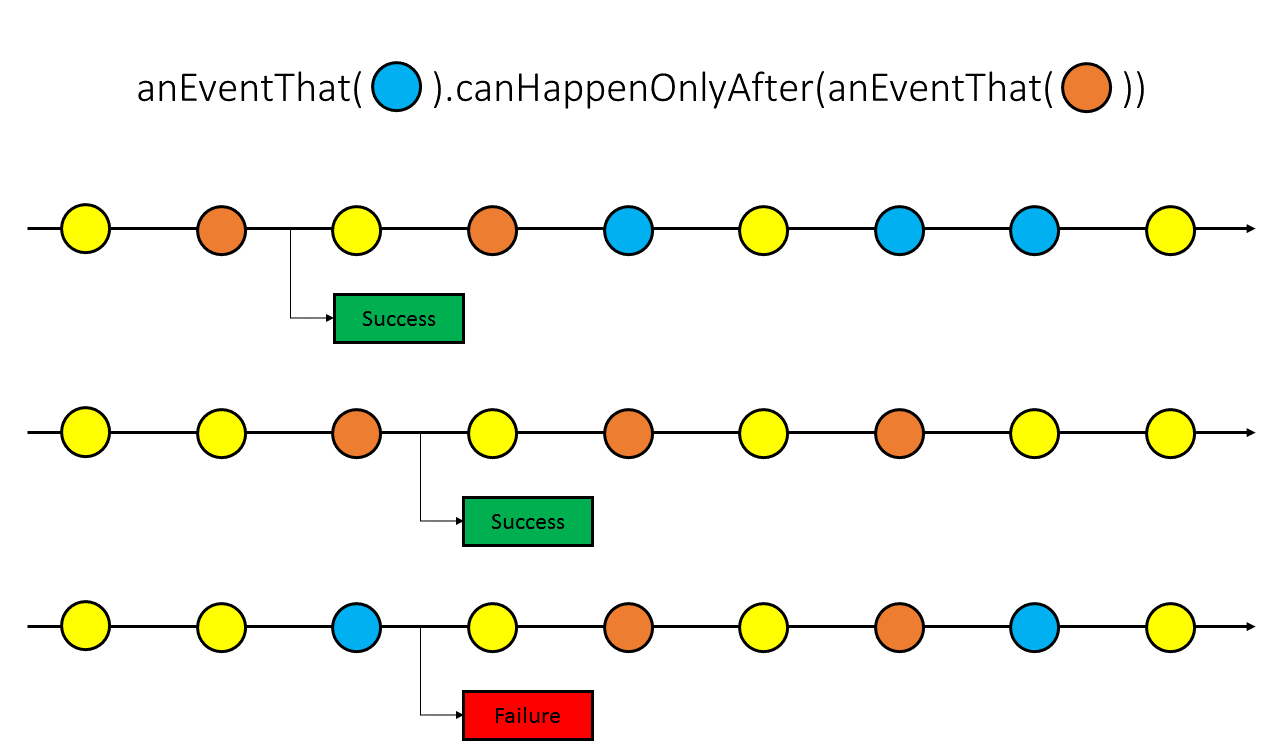
\includegraphics[width=400px]{Images/Language/CanHappenOnlyAfter.png}}
	
	Note in particular that in the second case the checks succeeds even if no blue event occurs: we are  just saying that blue events \textit{can} happen after an orange one.
	
  	\\ \hline
  	
  \rotatebox[origin=c]{90}{\textbf{ Code Example }} & 
  
  	\begin{lstlisting}
	anEventThat(isMarkerPlacement())
		.canHappenOnlyAfter(anEventThat(isMapReady()))
	\end{lstlisting}
	
  	\\ \hline  	
  	 
\end{longtable}
\egroup
\end{center}

\subsection{Checks on Sets of Events}

\subsubsection{Must Happen After}

\begin{center}
\bgroup
\def\arraystretch{1.5}%
\begin{longtable}{ | m{0.3cm} | m{15cm} | }
  \hline
  
  \rotatebox[origin=c]{90}{\textbf{ Structure }} & 
  
  	\begin{lstlisting}
	exactly(n).eventsWhereEach(m1).mustHappenAfter(anEventThat(m2))
	\end{lstlisting}
	
  	\\ \hline
  	 
  \rotatebox[origin=c]{90}{\textbf{ Description }} & 
  
  	Checks that exactly \texttt{n} events that match \texttt{m1} happen exclusively after every event that matches \texttt{m2}. "Exclusively" means that there cannot be another event that matches \texttt{m2} before the sequence of \texttt{n} events is completed.
	
  	\\ \hline

  \rotatebox[origin=c]{90}{\textbf{ FOL }} & 
  
  	\begin{multline*}
	\forall e2 \Bigg( match(e2, m2) \Rightarrow \exists_n e1 \bigg( match(e1, m1) \land before(e2, e1) \\ \land \neg \exists e2' \Big( match(e2', m2) \land between(e2, e2', e1) \Big) \bigg) \Bigg)
	\end{multline*}
	
  	\\ \hline

  \rotatebox[origin=c]{90}{\textbf{ Visual }} & 
  
	\raisebox{-280pt}{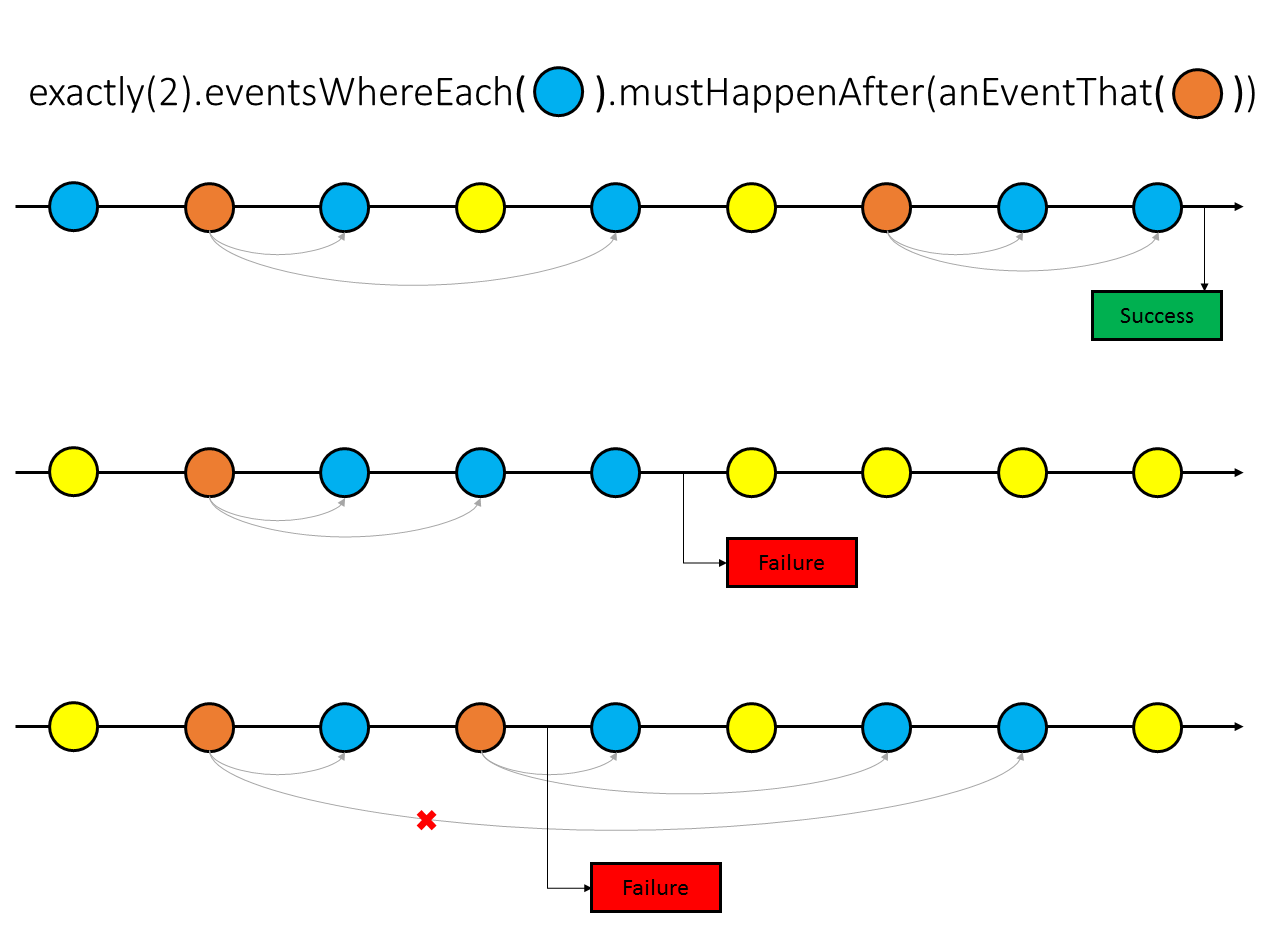
\includegraphics[width=400px]{Images/Language/MustHappenAfter.png}}
	
	Note in particular that the third case shows the "exclusively" constraint mentioned before: the check fails because we do not have two blue events after the first orange but before the second one (i.e. the first orange event does \textit{not} match one of the three blue events that follow the second orange event)

  	\\ \hline
  	
  \rotatebox[origin=c]{90}{\textbf{ Code Example }} & 
  
  	\begin{lstlisting}
	exactly(1).eventsWhereEach(isTextChangeFrom(locationTextView))
		.mustHappenAfter(anEventThat(isLocationChange()))
	\end{lstlisting}
	
  	\\ \hline  	
  	 
\end{longtable}
\egroup
\end{center}



\subsection{Checks on the Whole Stream}

\subsection{Connectives between Checks}



\section{Reactive Programming}

\subsection{ReactiveX}

\subsection{Components}

\subsection{RxJava and RxAndroid}

\subsection{Events Observable in Android}



\section{Design}



\section{Implementation}



\section{Evaluation}


%..............................................................................%
%................................. CONCLUSION .................................%
%..............................................................................%

\part{Conclusion}

\section{Recap}

\section{Future Work}


%..............................................................................%
%.................................. REFERENCES ................................%
%..............................................................................%

\bibliographystyle{plain}
\bibliography{} 

\end{document}


